\chapter[Materiais e Métodos]{Materiais e Métodos}

Na busca de uma solução para o sistema proposto, desmembrou-se o diagrama (Figura \ref{fig:blocos}) a fim de modularizar o processo. A aquisição, envio e recepção dos dados, assim como as especificações de comunicação (número de portadoras, tipo de modulação, codificação de linha e canal) não foram tratados neste trabalho. 


\begin{figure}[h]
	\centering
	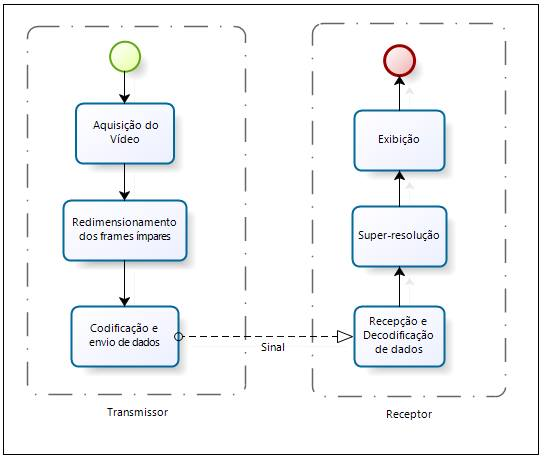
\includegraphics[scale=.7]{figuras/diagrama_blocos_solucao.jpg}
	\caption{Diagrama de blocos proposto para solução.}
	\label{fig:blocos}
\end{figure}

Implementou-se os blocos de redimensionamento dos \textit{frames} ímpares, que se dá no transmissor, pelo processo de filtragem (entre quadros pares e ímpares) e  decimação por um fator $M$ destes \textit{frames}, e o bloco de super-resolução, que se dá no receptor, que consiste na implementação do algoritmo proposto na Seção \ref{algPropos}. 

\section{Transmissor}

\subsection{\textit{Hardware}}
Para o transmissor, escolheu-se o \textit{kit} de desenvolvimento \textit{Raspberry Pi 2 Model B}, mostrado na Figura \ref{fig:rasp}. O \textit{Raspberry Pi 2} é um dos dispositivos mais populares atualmente entre estudantes, profissionais e hobbistas da área de Eletrônica. Segundo o próprio site da \textit{Raspberry Pi Foundation} \cite{raspberryOrg}, o dispositivo é um computador de dimensões reduzidas e de baixo custo, capaz de se conectar a um monitor de computador ou televisão e  rodar um sistema operacional baseado em Linux, sendo um dos mais populares o \textit{Raspbian} (distribuição \textit{Debian} voltada especificamente para o \textit{Raspberry Pi}).

\begin{figure}[h]
	\centering
	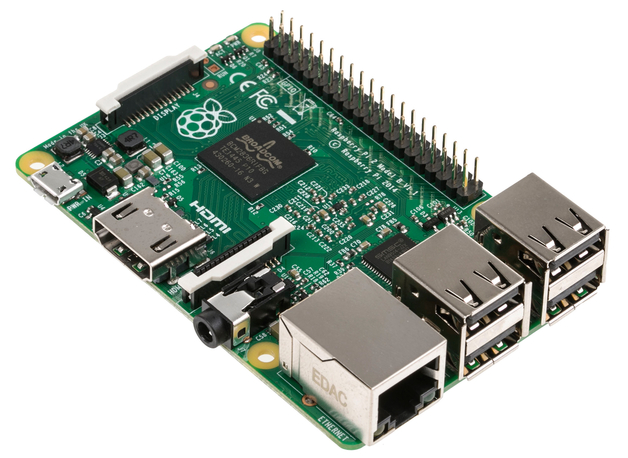
\includegraphics[scale=.5]{figuras/rpi2b.jpg}
	\caption{ \textit{Kit} de desenvolvimentoto \textit{Raspberry Pi 2 Model B} \cite{element14}.}
	\label{fig:rasp}
\end{figure}

A capacidade de rodar sistemas operacionais baseados em distribuições Linux foi uma característica decisiva na escolha do \textit{kit} de desenvolvimento, pois dá ao desenvolvedor a possibilidade de utilizar \textit{frameworks} e \textit{codecs} já disponíveis no mercado, além da alta capacidade de processamento disponível dos quatro núcleos ARM (\textit{Advanced RISC Machine}) e do processador gráfico dedicado. Há também módulos de aquisição e exibição de vídeo desenvolvidos e otimizados especialmente para a arquitetura deste dispositivo, o que pode facilitar o desenvolvimento futuro do bloco de aquisição e possibilitando a exibição local caso necessária. Segue um apanhado geral das características desta placa  \cite{raspberryOrg} :
\begin{itemize}
\item CPU de quatro núcleos ARM Cortex-A7 com frequência de processamento de 900 MHz;
\item  1 GB de memória RAM (contra 512 MB do modelo B+);
\item 4 portas USB;
\item 40 pinos GPIO (do inglês,\textit{General Purpouse Input/Output});
\item Porta Full HDMI;
\item Porta \textit{Ethernet};
\item Audio jack de 3.5mm e entrada de vídeo combinados;
\item Interface de câmera (CSI);
\item Interface para display (DSI);
\item Slot para Micro cartão SD;
\item Núcleo de gráficos VideoCore IV 3D;
\end{itemize}

Dentre os 40 pinos GPIO, têm-se pinos com funções dedicadas como: tensões de entrada e referência, além de diversos tipos de comunicações (I2C, SPI, serial, etc), como mostrado na Figura \ref{fig:rasp_gpio}.

\begin{figure}[h]
	\centering
	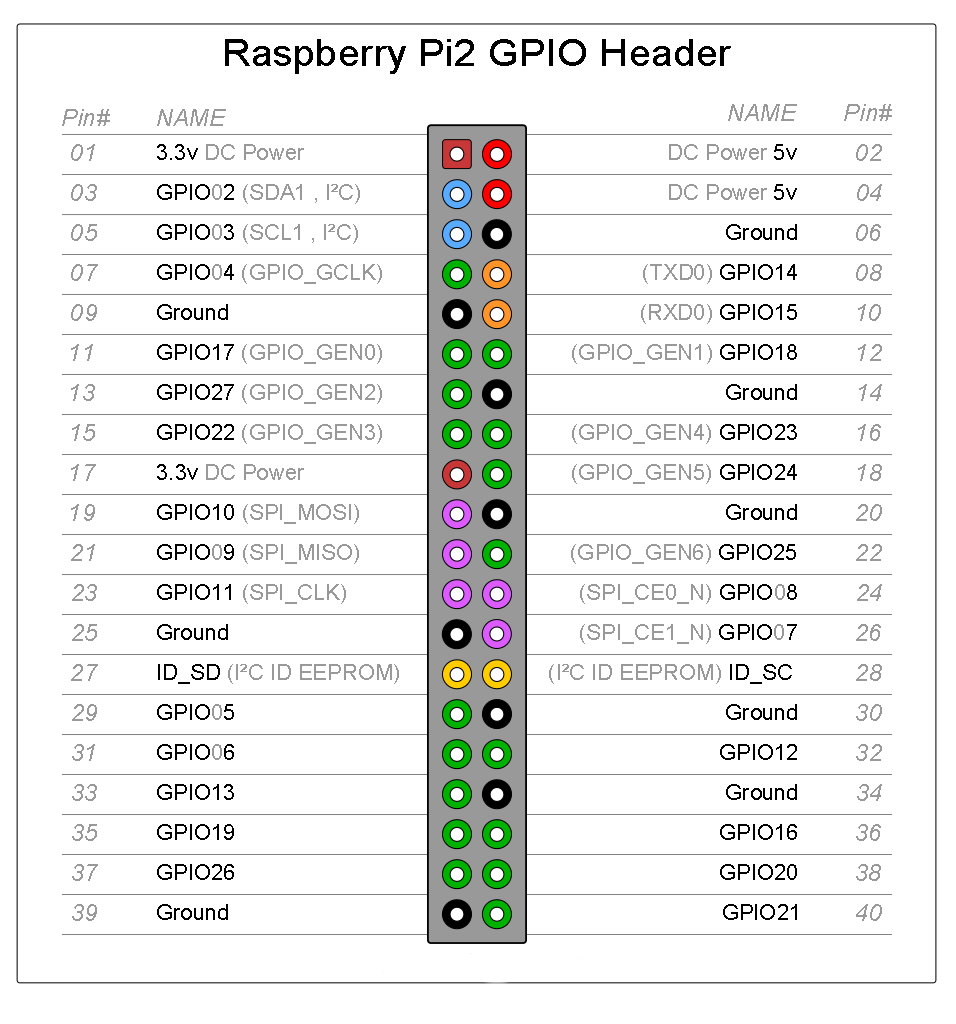
\includegraphics[scale=.3]{figuras/GPIO_Pi2.png}
	\caption{ Mapa de pinos do \textit{Raspberry Pi} 2 Modelo B \cite{element14}.}
	\label{fig:rasp_gpio}
\end{figure}

Assim, optou-se por utilizar \textit{Raspberry Pi2 Model B}, rodando um sistema operacional \textit{Arch Linux Arm}, em um cartão micro SD de 8 Gb,  com um \textit{Python} versão 2.7.
Utilizou-se o editor de texto \textit{Vim}, assim como conceitos de orientação a objetos e o \textit{multimedia framework} FFmpeg versão 2.8.2, fazendo uso principalmente do \textit{FFmpeg Tools}, uma ferramenta que permite redimensionar, codificar e converter vídeos em diversos formatos e um \textit{framework} de versionamento de código Git versão 2.1.4 .
\subsection{\textit{Software}}

No transmissor trabalhou-se na separação e redimensionamento dos quadros ímpares e, também na compressão das sequências de vídeo. Para isso, desenvolveu-se um \textit{script} na linguagem \textit{Python}, com utilização de \textit{FFmpeg}, um \textit{multimedia framework} de código aberto, que por sua vez, é  capaz de codificar e decodificar em diversos padrões, incluindo os dois propostos no trabalho (JPEG e H.246/AVC). Optou-se por essa linguagem devido a alta integração com o \textit{hardware} proposto, integração com \textit{frameworks} para cálculos cientificos (\textit{SciPy}) e experiência prévia do desenvolvedor. 

    A taxa de transmissão é controlada a partir de parâmetros relacionados ao coeficiente de quantização citado nas Seções \ref{JPEG} e \ref{H264}, que definem o nível de quantização utilizado no processo. 

\section{Receptor}

\subsection{\textit{Hardware}}

    Dentro do contexto proposto neste trabalho, o receptor terá amplos recursos de computação e energia, pois ele estará na superfície da mina. Já o transmissor estará exposto às condições adversas de dentro da mina. Assim, para o protótipo proposto neste trabalho, utilizou-se um computador pessoal com as seguintes configurações: um \textit{notebook} Asus X44C-VX029R - Intel Core i3-2330M - RAM 4GB - HD 320GB, rodando um sistema operacional \textit{Debian} 8 (Jiessie), com um \textit{GNU Octave}, versão 3.8.2. Utilizou-se também \textit{multimedia framework} \textit{FFmpeg} versão 2.8.2, fazendo uso principalmente do \textit{FFmpeg Tools}, uma ferramenta que permite redimensionar, codificar e converter vídeos de diversos formatos e um \textit{framework} de versionamento de código Git versão 2.1.4 . 


\subsection{\textit{Software}}

    A implementação do algoritmo de super-resolução proposto para o decodificador foi feita na linguagem \textit{Octave}, versão 3.8.2, pois ela é otimizada para o trato de matrizes e também devido à experiência prévia do desenvolvedor. O script desenvolvido recebe como entrada as sequências de vídeo vindas do transmissor, e gera as sequências de vídeo super-resolvidas com base no algoritmo apresentado no Capítulo anterior.

